\documentclass[tikz,border=8pt]{standalone}
% Shared look for every TikZ diagram. Load with \input{../../tools/tikz-style.tex}
\usepackage[T1]{fontenc}
\usepackage{lmodern}
\renewcommand{\sfdefault}{lmr}  % diagrams use the same serif as the text
\usetikzlibrary{arrows.meta, positioning, shapes.geometric, calc, fit, backgrounds}
\definecolor{cblue}{HTML}{4C78A8}
\definecolor{corange}{HTML}{F58518}
\definecolor{cgreen}{HTML}{54A24B}
\definecolor{cred}{HTML}{E45756}
\definecolor{cpurple}{HTML}{B279A2}
\definecolor{cgrey}{HTML}{6B6B6B}
\tikzset{
  every picture/.style={font=\sffamily, line width=1.2pt},
  box/.style={draw=#1, fill=#1!12, rounded corners=4pt, align=center, inner sep=7pt, minimum height=1.1cm},
  box/.default=cgrey,
  arrow/.style={-{Stealth[length=3mm]}, draw=cgrey, line width=1.4pt},
  title/.style={font=\sffamily\bfseries\Large},
  note/.style={font=\sffamily\small, text=cgrey, align=center},
}
\AtBeginDocument{\hyphenpenalty=10000 \exhyphenpenalty=10000}

\usetikzlibrary{matrix}
\begin{document}
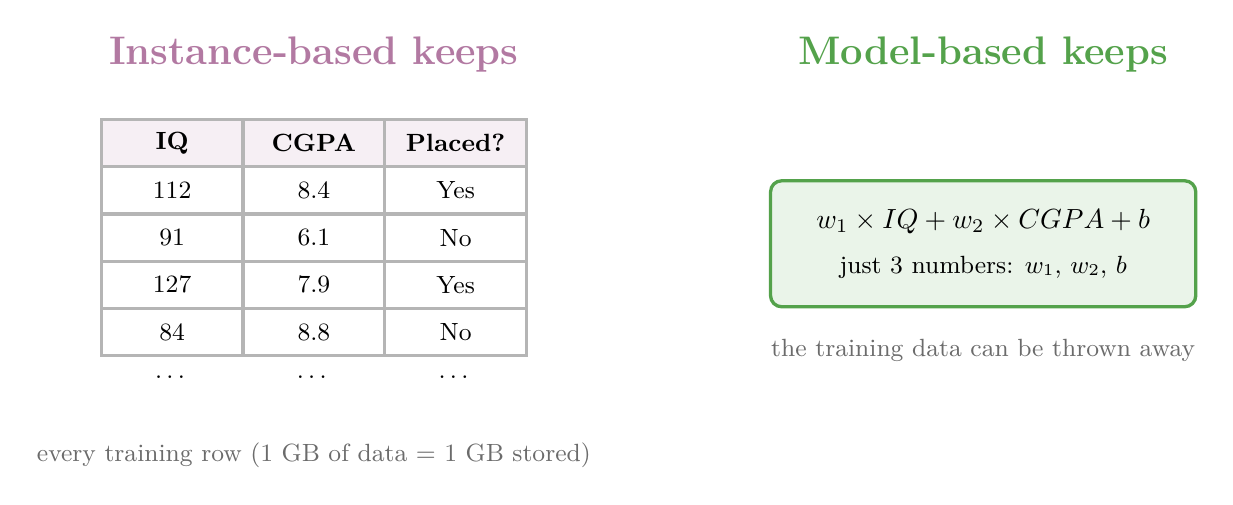
\begin{tikzpicture}
  \node[title, cpurple] at (0,2.6) {Instance-based keeps};
  \matrix (t) at (0,0) [matrix of nodes, column sep=-\pgflinewidth, row sep=-\pgflinewidth, nodes={minimum width=1.8cm, minimum height=0.6cm, anchor=center, draw=cgrey!50, font=\small},
      row 1/.style={nodes={font=\small\bfseries, fill=cpurple!12}}]
  { IQ & CGPA & Placed? \\ 112 & 8.4 & Yes \\ 91 & 6.1 & No \\ 127 & 7.9 & Yes \\ 84 & 8.8 & No \\
    |[draw=none]|\dots & |[draw=none]|\dots & |[draw=none]|\dots \\ };
  \node[note, below=0.25cm of t] {every training row (1 GB of data = 1 GB stored)};
  \node[title, cgreen] at (8.5,2.6) {Model-based keeps};
  \node[box=cgreen, minimum width=5.4cm, minimum height=1.6cm, align=center] (m) at (8.5,0.2)
    {$w_1 \times \text{IQ} + w_2 \times \text{CGPA} + b$\\[4pt]{\small just 3 numbers: $w_1$, $w_2$, $b$}};
  \node[note, below=0.25cm of m] {the training data can be thrown away};
\end{tikzpicture}
\end{document}
